% 95-40(95쪽) — 항구 $\pt{A}$ → $\pt{C}$ → 항구 $\pt{B}$ 의 항로(원문 「오른쪽 그림」). 스캔 화질이 낮아 TikZ 로 다시 그림.
% 라벨은 원문 것만: $10\,\mathrm{km}$·$6\,\mathrm{km}$·$14\,\mathrm{km}$·$\theta$ 와 $\pt{A}$·$\pt{B}$·$\pt{C}$, 그리고 $\pt{C}$ 에서 동쪽으로 뻗은 점선.
% 원문의 바다·항구 삽화는 수학 내용이 아니라 옮기지 않았다. $\theta$ 의 값(답)은 적지 않는다.
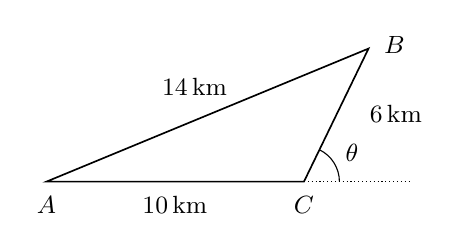
\begin{tikzpicture}[line width=0.6pt]
  \draw[densely dotted, line width=0.4pt] (3.27,0) -- (4.60,0);
  \draw (0,0) -- (3.27,0) -- (4.09,1.69) -- cycle;
  \draw[line width=0.4pt] (3.72,0) arc (0:64.1:0.45);
  \node[font=\small] at (3.88,0.36) {$\theta$};
  \node[anchor=north, font=\small] at (1.63,-0.06) {$10\,\mathrm{km}$};
  \node[anchor=west, font=\small] at (3.98,0.86) {$6\,\mathrm{km}$};
  \node[font=\small] at (1.88,1.20) {$14\,\mathrm{km}$};
  \node[anchor=north, font=\small] at (0,-0.06) {$\pt{A}$};
  \node[anchor=north, font=\small] at (3.27,-0.06) {$\pt{C}$};
  \node[anchor=west, font=\small] at (4.16,1.73) {$\pt{B}$};
\end{tikzpicture}
